\chapter{Preliminaries}
\label{Preliminaries}
\section{Graph Notations}
\begin{mydef}
A graph $G$ ist defined by a tuple $(V,E)$ with $V$ being a set of Verticies and $E$ a set of Edges.
$V = (v_{1}, ..., v_{n})$
\begin{enumerate}
 \item A graph is directed if the elements in $E$ consists out of tuples.\\
 $E = \{(v_{i},v_{j}),..\}$ for $v_{i},v_{j} \in V$ with $v_{i} \neq v_{j}$
 \item A graph is undirected if the elements in $E$ consists out of sets with the size of 2.\\
 $E = \{\{v_{i},v_{j}\},..\}$ for $v_{i},v_{j} \in V$ with $v_{i} \neq v_{j}$
\end{enumerate}
\end{mydef}
This definition is based on \cite{Diestel.2012}. If $\{v_{i},v_{j}\} \in E$ then $v_{i}$ and $v_{j}$ are neighbors. In a directed graph the direction of the edge matters, if $(v_{i},v_{j}) \in E$ then $v_{i}$ is a neigbor of $v_{j}$, but not the other way around.
\begin{mydef}
A graph $G$ is called a
\begin{enumerate}
 \item Multigraph if it contains multiple edges between the same vertices or edges from a vertex to the same vertex.
 \item Hypergraph if it contains edges, which have more than two vertices connected to it.
\end{enumerate}
\end{mydef}
\newpage
\section{Graph File Formats}
A graph file is a file, which contains the information to construct a Graph $G$.\\
Based on a the collection of graph file formats by \cite{Roughan.10.03.2015}.The most relevant file formats where chosen to be featured in this work. Relevant formats are formats that have been used in the recent time and still seem up-to-date, which is indicated by the overall use counts. Also, the amount of sample data of this file formats that can be found matters. File formats that don’t provide any clear specifications won’t be chosen either, duo to the fact that implementing them would result in a non-consistent parsing/reading, duo to missing constrains. This is based on the problem that other people don't have any specifications either. This could result in the missing conformity of their files. This work will try to select atleast one of each structure type to provide an example implementation of each structure type of graph file formats, so the amount of supported graph file formats can be extended easily.
\begin{table}[H]
\begin{center}
    \begin{tabular}{| l | l | l | l |}
    \hline
	\bfseries Id & \bfseries Graph File Format & \bfseries Reference Time Frame & \bfseries Structure\\ \hline
	1 & bintsv4 (GraphLab) & 2009 - 2015 & Simple binary\\ \hline
	2 & Dot & 2000 - present & BNF\\ \hline
	3 & Graph::Easy & 2004 - present & intermedia\\ \hline
	4 & GraphML & 2000 - present & XML\\ \hline
	5 & JSON Graph & 2014 - present & JSON\\ \hline
	6 & KrackPlot & 1993 - present & simple\\ \hline
	7 & Matlab & 1996 - present & HDF5\\ \hline
	8 & Ordered Graph Data Language & 2002 - present & BNF\\ \hline
	9 & Open Graph Markup Language & 2012 - present & XML\\ \hline
	10 & Simple Interaction Format & 2003 - present & simple\\ \hline
	11 & Stanford Network Analysis Platform & 2005 - present & simple\\ \hline
	12 & So NIA Son format & 2002 - present & intermedia\\ \hline
	13 & Trival Graph Format & NA - NA & simple\\ \hline
    \end{tabular}
\end{center}\caption{Selection of Graph File Formats based on\cite{Roughan.10.03.2015}}
\label{tabelle_avarage_time}
\end{table}

\subsection{Divisibility}
One of the main topics of this work is to increase the loading speed, by dividing large files into smaller chunks and load them on multiple peers at once. To archive that the file format must be able to be divided into such chunks. Otherwise a distributed loading isn’t possible and a single peer solution will be the best option.\\
Most of the file formats are divisible in some sort but the fastest way to split files is without or minimal reading of the file. So, the files still need to be dividable, if most of the information is skipped. Skipping most likely won’t be an option for all formats but for the simple and trivial ones it definitely will be.\\
To determine if a format is divisibility the structure of the file needs to be specified and analyzed. Most important data inside the file shouldn’t be dependent on other sections of the file. Sure, there will be formats that specify information about vertices in multiple sections of the file, but this information need to be independent. If the following data can only be processed after processing all lines before, then this section can be split. Eespectively this sections appear very often because most  key/values-tuples can’t be split. This section will be called contiguous regions of a file.\\
These contiguous regions are often closed of by separators. An seperator could be anything often newline characters, tabulations and  semicolons are used, but also tags (XML), brackets (JSON) or even the position itself in binary sequences can be used to divide these sections. Some formats provide metadata, that will help split up files by defining the position of the information and their format.\\
A format is fully divisible if it could be split at the any seperator. This definition is deliberately vague, because many test cases can be constructed to defeat certain characteristics.

\subsection{Simple Formats}
Simple formats can be often referred to as formats that provide a trivial approach to create a graph format. Often no specification is provided and it isn’t clear where the boundaries of this formats are, like the range of integer values, which character set is used or if the format contains metadata/comments. Many of these formats are fully dividable, duo to the fact that they often contain only one contiguous regions and have a plain hierachy. Also only one seperator is used, so that spkitting at every seperator is given.\cite{Roughan.10.03.2015}
\newpage
\subsubsection{Trivial Graph Formats}
As trivial graph file formats (TGF) are referred to a list of formats that vary by every implementation. Standard approaches are edge list, adjacency matrices, neighbor lists and path list.
Most of the lines inside a simple edge list are the same list just connections between node a and node b separated by tabs, comma or spaces. It is clear that this format can be split easily by just jumping to a position and reading till the next line. All following data could be a new chunk, same approaches can be applied to adjacency matrices, neighbor lists and path list.\\
The SNAP format is very similar to an edge list with the only addition that comments can be added to the file with a hash tag at the beginning of the line, that’s why it is group with the TGF.\\
In all these formats lines can be seen as contiguous regions and only one seperator is used, in fact newline characters are the most common separator for TGF. 

\begin{figure}[H]
	\centering
	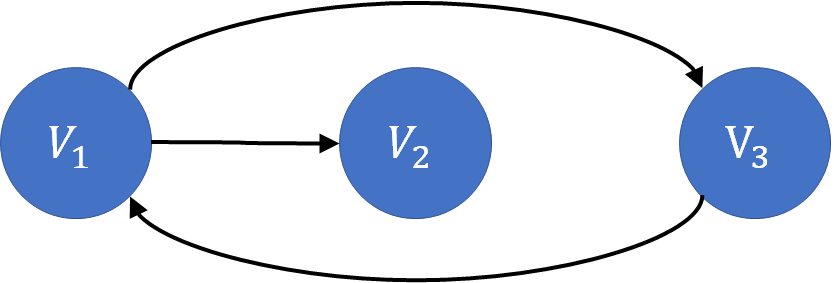
\includegraphics[height=4cm]{img/simple.png}
	\label{simple}
		\setlength{\tabcolsep}{0.5cm} % Abstand zwischen den Spalten einer Tabelle
		\begin{tabular}{lllll}
			\\
			adjacency matrices & neighbor list & edge list & path list \\
			$A = \left( \begin{array}{rrr}0 & 1 & 1 \\0 & 0 & 0 \\1 & 0 & 0\\\end{array}\right)$ &$\begin{array}{lll}1, 2\\1, 3\\3, 1\\\end{array}$ &$\begin{array}{lll}1: & 2,3 \\ 2: \\ 3: & 1\\\end{array}$ &$\begin{array}{lll}3,1,2 \\ 1,3 \\\end{array}$ \\
			
		\end{tabular}
	\caption{An example graph with three vertices in different trivial graph formats\cite{Roughan.10.03.2015}}
\end{figure}

		

\subsubsection{SIF Format}
The SIF Format is a combination of an edge list with a neighbor list. Additionally, the type of connection can be specified with strings. It allows multiple edges between the same nodes, if the connection type varies, otherwise it is specified to ignore duplicates. This results in an Multigraph. One downside is that the format allows tabulations or spaces as separators, it is stated that if no tabulations are used in the whole file spaces are used as separators, but because all lines have an equal format, it can be stated, if the first line doesn’t contain any tab character, spaces will be used as separators. Based of the fact that SIF is merge of two TGFs, it can be said that SIF is also fully divisable, only one separator is used per file and the lines are the contiguous regions. \cite{TheCytoscapeConsortium.2017}

\subsubsection{KrackPlot 3.0}
KrackPlot 3.0 follows for simple formats a more complex syntax then the TGFs. The first line contains the number of nodes specified in the following data. This information helps with various problems, like splitting nodes appropriately into chunks. The next line can contain two options “!nc” or “!nl”. The first option specifies that the following data contains no coordinates, the other one declares that no labels will be specified. If labels and/or coordinates are defined they start on the second line until line (node-amount) +1. After the second line or the labels/coordinates an adjacency matrix specifies the connections of the nodes.
This design choices of the format, make reading huge files on multiple peers tedious, duo to the fact that labels and coordinates are split apart from one another. Also, the overhead of an adjacency matrix is huge for large files.
Splitting this file is possible duo to the fact that we know the number of nodes. Only two lines need to be read in to know the whole nature of the file, which can be split according to the metadata.\cite{D.KrackhardtJ.BlytheC.McGrath.4.12.2001}\\
This formats consists out of two different sections. These sections contain different contiguous regions. This format is fully divisible becausse the size of the sections is know. 

\subsection{XML Formats}
There are various implementations of graph file formats using XML. The XML format is based around tags, which define the object it is describing. XML was most popular in the 90s and it is a structure descriptive language. Reading its information is as result not line based rather it is tag based. This format is hard to divide without reading it completly, because the XML format conists of multiple layers. This results in the problem to determin the layer on which the object is located, this problem can only be solved by counting the opened and closed tags or using a flat hierachy.\cite{bray1997extensible,Roughan.10.03.2015}


\subsubsection{GraphML}
GraphML is an XML based graph file format. It consists out of one graph element which can contain unordered node and edge elements. GraphML supports hyperedges and nested networks. This results in the problem of deep hierachies, which can only be solved by tag counting do determin the layer. GraphML support many kinds of graphs, this variety causes many different cases to consider. GraphML doesn't specify the positions of vertices or edges inside the format, so that chunks could result in an unequal distrubution of different objects. As result GraphML isn't fully divisble and needs to be read chunk by chunk, no information can be skipped.\cite{brandes2013graph,kuhner2013graphml}

\subsubsection{Open Graph Markup Language}
The Open Graph Markup Language is part of the Open Graph Drawing Framework. The OPML got some similarities to GraphML, duo to the fact that both formats resolve around XML. Also, this format implements many graph style and drawing operations. Also the OPML doesn’t support nested graphs unlike GraphML.\cite{opengraph.format}

\subsubsection{Resource Description Framework}
The Resource Description Framwork/XML Format is format that features the model of three information types. RDF defines via namespaces objects and attributes, which makes RDF a portable format, which got used to share graphs overtime and wasnt developed with this goal in mind.\cite{miller1998introduction,Lassila98resourcedescription}

\subsection{JSON Graph}
JSON Graph is unlike XML just a syntax convention based on the JSON-syntax-specification. This file format extends JSON files by introducing objects for graph description. These files are valid JSON-files and will be accepted by any JSON parser. Inside the JSON Graph file, a graph object is defined which contains nodes and edges with metadata. 
This format comes with a huge flaw, because the number of nodes, edges or any assistance to navigate inside the file with our reading it until that point isn’t given. Nodes and edges can span over multiple lines and don’t have a fixed size in any way. Metadata is expandable without any limits. The result of this design choice is that the file needs to be read sequentially before splitting it up into chunks. This will result in a huge performance loss.\\
One way of reading this format into memory while also using our maste/slave-system would be filling a buffer with the information read. And after that sending it to the processing slave.\cite{json.format,Roughan.10.03.2015}

\subsubsection{Other Formats}
This thesis can't deal with all graph formats that are available. For those cases the application will provide an API to extend its range of covered graph file formats.